\documentclass[journal, a4paper]{IEEEtran}
\usepackage[utf8]{inputenc} %UTF8 input file
\usepackage[T1]{fontenc}
\usepackage[ngerman]{babel} %Umlaute,Silbentrennung
\usepackage{amssymb} %triangleright
\usepackage{enumitem} %itemize einrücken 
\usepackage{graphicx} %Grafiken einbinden
\usepackage{booktabs} %Tabellen
\usepackage{caption}
\usepackage{amsmath}
\usepackage{epstopdf}
%\usepackage{natbib}
%\usepackage[nottoc,notlot,notlof]{tocbibind} %Bib to TeX
\date{\today}
\author{Malte~Ollenschläger}
\title{DIY: Herstellung eines personalisierten Weckers mit Mikrocontroller und mp3-Player}
\begin{document}

\maketitle
\begin{abstract}
	Dieses Dokument beschreibt die Herstellung eines personalisierten Weckers. Das beinhaltet die Erstellung eines Gehäuses und das Schreiben der Software für den Mikrocontroller. Auch die Bauteilauswahl und die Fertigung von Platinen sind in diesem Projekt inbegriffen. Das Ziel ist einerseits die Fertigung des Weckers, andererseits die Durchführung eines Projektes mit verschiedenen Aufgabenbereichen, um das hierbei Gelernte, in folgenden Projekten zu einer effizienteren Arbeitsweise umzusetzen. Dies betrifft sowohl inhaltliche als auch formelle Arbeitsschritte.
\end{abstract}

%\begin{IEEEkeywords}
%mp3-Wecker,
%\end{IEEEkeywords}

\section{Zielsetzung}
	\IEEEPARstart{D}{ie} Gesamtfunktion des Weckers soll sich aus mehreren Teilfunktionen zusammensetzen. Eine der grundlegenden Funktionen ist die Anzeige der Uhrzeit auf einem Display. Weiterhin wird das Datum durch die Zusammensetzung des aktuelle Monats als Wort und des Tages als Ordinalzahl angezeigt. Für den Monat Februar sollen Schaltjahre berücksichtig werden. % An ausgewählten Tagen, wie zum Beispiel dem der Besitzerin soll das Display anstatt des Datums eine andere \textit{Zeichenkette oder ein Bild} anzeigen.
	Ein weiteres Symbol gibt an, ob der Alarm ein- oder ausgeschaltet ist. Das De- beziehungsweise Aktivieren des Alarms geschieht durch das Gedrückthalten eines Tasters, über den gleichzeitig bei kurzem Drücken die die Beleuchtung eingeschaltet werden kann. Die Implementierung der Weckfunktion sorgt bei eingeschaltetem Alarm dafür, dass zur konfigurierten Uhrzeit der mp3-Player gestartet und eine sich auf selbigem befindliche mp3-Datei über die verbauten Lautsprecher wiedergegeben wird. Beim nächsten Weckruf wird die darauf folgende Datei abgespielt.\par

	Über ein Menü, das über das Bedienen eines zweiten Tasters zu erreichen ist, sind folgende Elemente einstellbar:
	\begin{itemize}[leftmargin=20mm]
	\item Uhrzeit
	\item Weckzeit
	\item Datum
	\item Lautstärke
	\item Boombox
%	[$\blacktriangleright$]
	\end{itemize}
	Innerhalb des Menüs findet die Navigation über einen Drehencoder statt. Wird der Menüpunkt \textit{Boombox} ausgewählt, so kann über ein Cinch-Kabel eine externe Audio-Quelle angeschlossen werden und die darauf abgespielte Musik wird über die Lautsprecher des Weckers wiedergegeben.\par
	Die Personalisierung des Weckers wird durch drei Eigenschaften erreicht. Die erste ist die Tatsache, dass die Weckmusik nach dem eigenen Geschmack angepasst werden kann, indem diese auf den mp3-Player kopiert wird. Die zweite personalisierte Eigenschaft ist, dass beispielsweise an Valentinstag und am Geburtstag der Person statt des Datums andere Bilder oder Texte eingeblendet werden. Der offensichtlichste Teil der Personalisierung liegt in der Herstellung des Gehäuses. In die Front des Weckers werden Motive gelasert zu denen die Benutzerin einen persönlichen Bezug hat. Diese werden zusätzlich zum Display beleuchtet, wenn der entsprechende Taster betätigt wird.
	Als Vorlage für dieses Projekt diente ein ebenfalls selbst hergestellter Wecker, der auf der Internetseite www.wiesolator.de vorgestellt wurde.\par
	Alle im Rahmen dieses Projekts erstellten Dateien sind unter \emph{www.github.com/MalteBastelt/Wecker} zu finden.
	
\section{Hardware}
	Dieser Abschnitt befasst sich mit der gesamten Hardware des Weckers. Hierzu wird in Teil \ref{sc:Hardware:subsc:Bauteile} beschrieben, welche Bauteile benötigt werden. Der sich anschließende Teil \ref{sc:Hardware:subsc:Dimensionierung} befasst sich mit der externen Beschaltung der Bauteile. Es folgt ein Abschnitt über die Pinbelegung am Mikrocontroller in \ref{sc:Hardware:subsc:Pinbelegung}. Abschnitt \ref{sc:Hardware:subsc:mp3-Player} beschreibt die Ansteuerung des mp3-Players. In \ref{sc:Hardware:subsc:Platinen} wird auf die Planung und Fertigung der Platinen eingegangen. Weiterhin erläutert \ref{sc:Hardware:subsc:Gehäuse} die Herstellung des Gehäuses.
	
	\subsection{Bauteile}
		\label{sc:Hardware:subsc:Bauteile}
		Der Schaltplan, der im Vorlageprojekt genutzt wurde, dient als Anhaltspunkt für die Hardware, die benötigt wird. Daraus wurde das Schaubild in Abb. \ref{fig:Hierarchie} erstellt, um eine Übersicht der wichtigsten Bauteile zu erhalten.
		\begin{figure}
				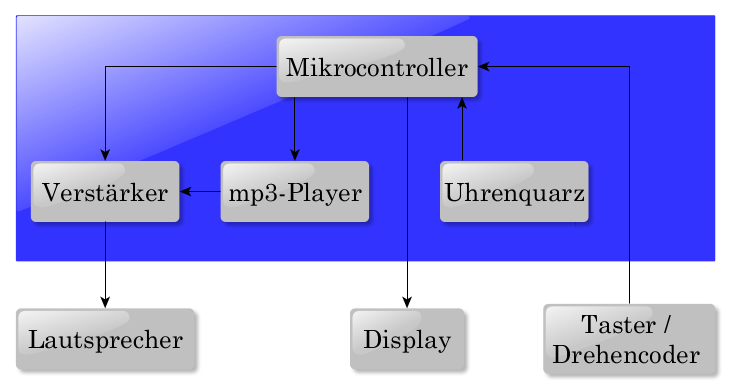
\includegraphics[width=80mm]{./Grafiken/Hierarchie}
				\caption{Hierarchie der Elementaren Bauteile des Weckers. Die Pfeilspitze zeigt in die Datenflussrichtung. Blau unterlegt sind die für den Benutzer nicht zugänglichen Bauteile im Gehäuse. Die unterste Zeile zeigt die Ein- und Ausgabeebene, worüber der Benutzer mit dem Wecker interagiert.}
				\label{fig:Hierarchie}
		\end{figure} 
		Eine Auflistung aller benötigter Bauteile ist in Tabelle \ref{tab:Bauteile} aufgeführt. Die benötigten Widerstände und Kondensatoren sind nicht aufgeführt, da diese den Datenblättern der jeweiligen Bauteile zu entnehmen sind. 
		\begin{center}
			\begin{tabular}{rl}
				\toprule
				Funktionseinheit & Bezeichnung \\
				\midrule
				Buchsenleiste & EBLG-20-1-X\\
				Display & EA DOGL128W-6 \\
				Displaybeleuchtung & EA LED68x51-W\\
				Drehencoder & STEC11B \\
				Lautsprecher & Visaton FR8-8 \\
				Leuchtdioden & DLE-0000397\\
				Mikrocontroller & Atmega328P \\
				mp3-Player & Intenso Music Walker \\
				Plexiglas & \\
				Schaltnetzteil 5V/1A & goobay 54805 \\
				Spannungsregler 1,5VDC & LM317\\
				Spannungsregler 3,3VDC & LM3940 \\
				Spanplatten & \\
				Schrauben &\\
				Muttern&\\
				Taster & MS 131 SW \\
				Transistor & BC547C \\
				Transparenzfolie & \\
				Uhrenquarz 32kHz& - \\			
				Verstärker & TDA7266 \\
				\bottomrule		
			\end{tabular}
			\captionof{table}{Benötigte Bauteile. Notwendige Kondensatoren und Widerstände sind nicht angegeben. Diese sind in den jeweiligen Datenblättern zu finden.}
			\label{tab:Bauteile}
		\end{center}
		
	\subsection{Dimensionierung}
		\label{sc:Hardware:subsc:Dimensionierung}
		Grundsätzlich wurden die in den Datenblättern empfohlenen Kondensatoren und Widerstände eingesetzt. Zum Entprellen der Taster sind in den entsprechenden Datenblättern keine Informationen vorhanden. Es werden Keramikkondensatoren der Größe $C=100 nF$ genutzt. Bei dem Spannungsregler für den mp3-Player (LM317) muss eine individuelle Dimensionierung vorgenommen werden, da der Ausgang des gewählten Spannungsreglers variable Spannungen erzeugen kann.
		Die benötigte Versorgungsspannung beträgt $1,5 V$. Nach der im zugehörigen Datenblatt \cite{LM317} angegebenen Formel, kann für eine gewünschte Ausgangsspannung die Größe der benötigten Widerstände berechnet werden.  Somit ergibt sich die Größe von $R_2$ nach folgender Gleichung:
		\begin{equation}
			\label{eqn:1,5VDC}
			R_2 = (\frac{V_{out}}{V_{ref}}-1) / (\frac{1}{R_1}+I_{adj})
		\end{equation}	
		Für den Ausgleichsstrom wurden 50$\mu A$ und damit die Hälfte des Maximums angenommen. Dieser wird vom Spannungsregler so geregelt, dass $V_{ref} = 1,25 V$ gilt. Bei einer Wahl von $R_1 = 10k\Omega$ ergibt sich für $R_2 \approx 1,3 k\Omega$.\par
		Zur Beleuchtung der beiden Bilder auf der Frontseite des Weckers wird je Bild eine Transistorschaltung (Abb. \ref{fig:Transistor}) benötigt. 
		\begin{figure}
			\begin{center}	
				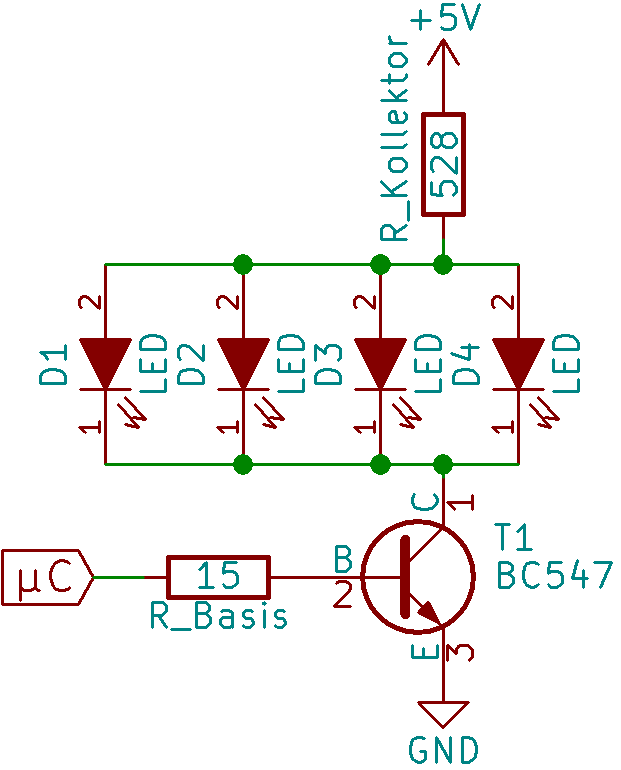
\includegraphics[width=5cm]{./Grafiken/Transistor.png}
				\caption{Transistorschaltung zur Ansteuerung von LEDs}
				\label{fig:Transistor}
			\end{center}
		\end{figure}
		Diese wird durch ein Kontrollsignal vom Mikrocontroller, welches an die Basis des Transistors angeschlossen ist, gesteuert. Ein BC547C Transistor schaltet vier LEDs. Der Kollektorstrom von $I_C$ ist das Vierfache des Vorwärtsstroms einer LED $I_F = 20mA$ \cite{LED}:
		\begin{subequations}
			\label{eqn:Kollektorstrom}
			\begin{align}
				I_C & = 4 \cdot I_F\\
				I_C & = 4 \cdot 20mA = 80mA
			\end{align}
		\end{subequations}
	  Dies folgt aus der ersten Kirchhoff'schen Regel, wonach sich der Kollektorstrom gleichmäßig auf die vier LEDs aufteilt. Die Berechnung der Widerstände ergibt sich aus folgen Formeln: 
		\begin{equation}
			\label{eqn:R_Basis}
			R_{Basis} \leq \frac{U_{\mu C}-U_{BE}}{I_B} =  \frac{3,3V-0,66V}{5mA} \approx 528\Omega
		\end{equation}
		\begin{equation}
			\label{eqn:R_Kollektor}
			\begin{split}
				R_{Kollektor} = & \frac{U_{cc}-U_{LED}-U_{CE}}{I_{C}} = \\ 
				&\frac{5V-3,6V-0,2V}{80mA} \approx 15\Omega
			\end{split}
		\end{equation}
		Da der Mikrocontroller eine Versorgungsspannung von $3,3V$ hat, ist das Steuersignal $U_{\mu C}$ ebenso groß. Die Basis-Emitter-Spannung $U_{BE}$ und die Kollektor-Emitter-Spannung $U_{CE}$ sowie der Basisstrom $I_B$ sind dem Datenblatt des BC547C entnommen \cite{BC547C}. Entsprechendes gilt für die an den LEDs abfallende Spannung. Nach den Berechnungen in den Gleichungen \eqref{eqn:Kollektorstrom} bis \eqref{eqn:R_Kollektor} wurde der Basiswiderstand zu $440\Omega$ und der Kollektorwiderstand zu  $15\Omega$ gewählt.

	
	\subsection{Pinbelegung Mikrocontroller}
		\label{sc:Hardware:subsc:Pinbelegung}
		Da es für den Oszillator keine Auswahlmöglichkeiten bezüglich der Pinbelegung gibt, wurden ihm als erstes die entsprechenden Pins am Mikrocontroller zugewiesen. Hierfür ist kein Datenblatt vorhanden, weil er im Einzelhandel ohne exakte Artikelbeschreibung gekauft wurde. Die Pins für den Anschluss des Displays wurden so gewählt, dass alle nebeneinander liegen, damit das Layout der Platine erleichtert wird und lediglich gerade Leiterbahnen zwischen den Pins des Mikrocontrollers und dem betreffenden Steckverbinder erstellt werden müssen. Gleiches gilt für die Belegung der Pins zur Ansteuerung des mp3-Players.\par
		Die Auswahl für die Belegung der Taster unterliegt lediglich der Einschränkung, dass die Taster (Licht und Drehencoder) einem anderen Interrupt zugeordnet werden als eine Drehung des Drehencoders. Dies führt zu einer vereinfachten Auswertung der Drehrichtung, siehe Abschnitt \ref{sc:Software:subsc:Atmel-Code}.
	
	\subsection{Ansteuerung mp3-Player}
		\label{sc:Hardware:subsc:mp3-Player}
		Um ein Bild davon zu bekommen, wie die Steuerung des mp3-Players funktioniert, wurde dieser zunächst aus seinem Gehäuse ausgebaut. Durch Testen wurde die Funktionsweise der benötigten Taster simuliert.  In Abb. \ref{fig:mp3-Player} ist eine Zeichnung des mp3-Players dargestellt, die zum näheren Verständnis des folgenden Textes herangezogen werden kann.\par 
		Der silberne Steuerknopf hat auf zwei gegenüberliegenden Seiten je 3 Kontakte. Darüber liegt rings um diesen Knopf unterhalb der Plastikabdeckung eine Massefläche. Wird der Knopf in eine bestimmte Richtung bewegt, so wird einer der 6 Pins auf Masse gezogen und daraus resultiert ein Steuersignal. Welches Ereignis durch die  verschiedenen Pins ausgelöst wird, ist in Tabelle \ref{tab:mp3-Player} dokumentiert. Zur Betätigung des Ein- und Ausschalters, der bei kurzem Drücken für Play/Pause genutzt wird, muss eine bestimmte der vier daran befindlichen Lötstellen auf das Level $1,5V$ gehoben werden. Zwei Lötstellen befinden sich auf der Oberseite und zwei in Richtung Mitte der Platine. Von letzteren muss die Lötstelle, welche in Richtung der $3,5mm$-Klinken-Buchse liegt, auf $1,5V$ angehoben werden. Um das $3,3V$ Schaltsignal des Mikrocontrollers auf $1,5V$ für den mp3-Player zu verringern, wurden 3 Dioden vom Typ 1N4448 in Reihe zwischen den Ausgang des Mikrocontrollers und den betreffenden Konnektor zum mp3-Player geschaltet. Über den Dioden fällt jeweils etwa $0,6V$ ab, sodass $3,3V-3\cdot0,6V = 1,5V$ an dem Taster anliegen, wenn der Pin des Mikrocontrollers auf $3,3V$ gesetzt ist. Die Versorgungsspannung des mp3-Players wird über einen $1,5V$-DC/DC Spannungsregler zur Verfügung gestellt.
		\begin{center}
			\begin{tabular}{ccc}
				\toprule
				Pin  &  Level & Ereignis \\
				\midrule
				1 & 0V & Song wechseln\\
				3 & 0V & Lautstärke -\\
				4 & 0V & Lautstärke +\\
				On-1 & 1,5V & Ein/Aus, Play/Pause\\
				\bottomrule		
			\end{tabular}
			\captionof{table}{Tastenkombination für Auslösung verschiedener Ereignisse. Funktion von On-1 je nach Betätigungsdauer (lang,kurz).}
			\label{tab:mp3-Player}
		\end{center}
		\begin{figure}
			\begin{center}
				\label{fig:mp3-Player}
				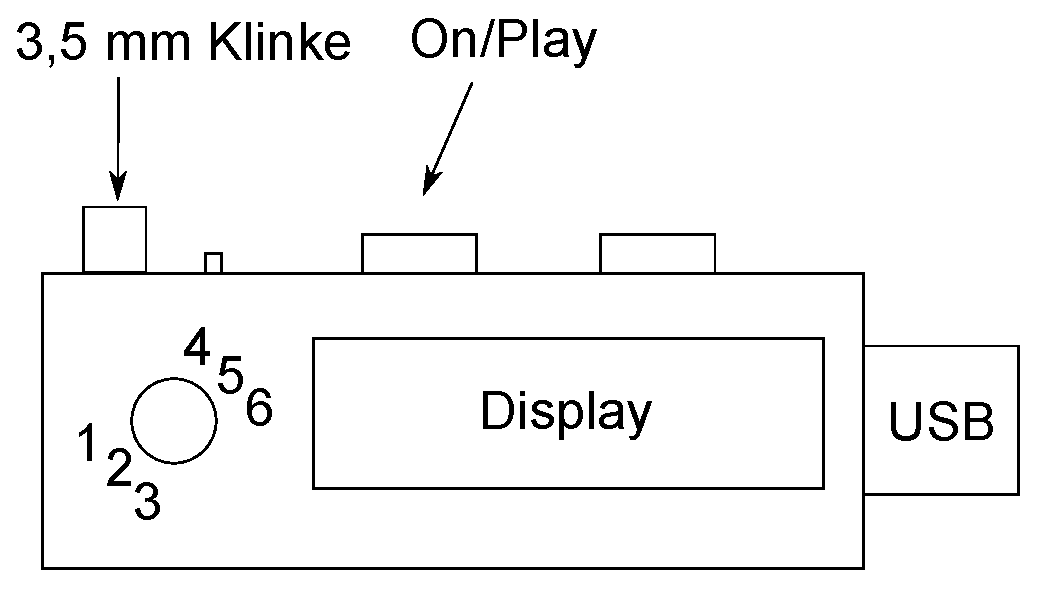
\includegraphics[width=5cm]{./Grafiken/mp3Player.eps}
				\caption{Pinbelegung mp3-Player}
			\end{center}
		\end{figure}
		
		\subsection{Platinen}
		\label{sc:Hardware:subsc:Platinen}
		Die für dieses Projekt benötigten Platinen wurden mit KiCAD geplant und anschließend im FabLab der Friedrich-Alexander-Universität Erlangen-Nürnberg erstellt. Die erste Platine konnte nicht verwendet werden, da das ausgedruckte Layout nicht den tatsächlichen Dimensionen entsprach. Die Ursache hierfür liegt vermutlich im Export des Schaltplans in eine PDF-Datei. Korrekte Maße bleiben nur Erhalten, wenn in eine PostScript-Datei anstatt in ein PDF exportiert wird.\par Eine Platine ist für das Display und die zugehörigen Bauelemente (Kondensatoren, Widerstände) ausgelegt. Über einen Steckverbinder kann diese Platine mit der Hauptplatine verbunden werden, welche die anderen Bauelemente wie zum Beispiel den Mikrocontroller und den Audio-Verstärker enthält. \par
		Für die Displayplatine wurden die Anschlüsse des Displays nicht direkt auf der Platine verlötet. Es wurden Buchsenleisten verlötet in welche das Display samt verlöteter Hintergrundbeleuchtung eingesteckt wird. Dies dient einerseits dazu, dass das Display zum Wechsel oder zur Reparatur ausgebaut werden kann; andererseits dazu, dass der Abstand zwischen Gehäuseinnenseite und Platine vergrößert wird. Dies ist notwendig, damit der Drehencoder, welcher auf der Platine befestigt wird, nicht zu weit nach vorne aus dem Gehäuse herausragt. Außerdem dient es der Herstellung einer kraftschlüssigen Verbindung zwischen Display und Gehäuse (siehe \ref{sc:Hardware:subsc:Gehäuse}).  Für die Erstellung der Platine wurde eine Leiterbahnbreite von $0,5mm$ gewählt, da genug Fläche vorhanden war.\par
		Für die Hauptplatine (Abb. \ref{fig:Hauptplatine}) wurde ebenfalls eine Leiterbahnbreite von $0,5mm$ gewählt. Neben der Displayplatine wurden weitere Bauelemente per Steckverbinder mit der Hauptplatine verbunden. Diese sind:
		\begin{itemize}
			\item Lautsprecher
			\item Taster
			\item Drehencoder
			\item LED-Beleuchtung (Bilder)
			\item mp3-Player
		\end{itemize}
		Für die Befestigung des Drehencoders wurde in die Displayplatine an der entsprechenden Position ein Loch gebohrt. Weiterhin erhielt die Platine in den vier Ecken je eine Bohrung, damit sie später mit Schrauben befestigt werden kann. Der Drehencoder ist ausreichend lang, sodass er aus der Front herausragt und bedient werden kann. Der Taster zur Bedienung der Beleuchtung wird in ein Loch passender Größe geklemmt.
		
		\begin{figure}
			\begin{center}	
				\includegraphics[width=8cm]{./Grafiken/Platine.jpg}
				\caption{Hauptplatine. Bauteilanordnung wie im KiCAD-Projekt (siehe Github-Verzeichnis).}
				\label{fig:Hauptplatine}
			\end{center}
		\end{figure}	
		
		\subsection{Gehäuse}
			\label{sc:Hardware:subsc:Gehäuse}
			Das Gehäuse wurde aus Spanplatten hergestellt. Um für ausreichend Stabilität zu sorgen, haben diese eine Stärke von $8mm$. Die sechs benötigten Elemente wurden mit einer Kreissäge der Firma Martin zugeschnitten. Hierbei ist es möglich, das Sägeblatt um bis zu $45^{\circ}$ zu neigen. Dies wurde genutzt, um die einzelnen Elemente auf Gehrung zu sägen. Die Schnittwinkel an jeder Kante ergeben sich aus dem halben Gesamtwinkel der jeweiligen Kante.
				\begin{figure}
					\begin{center}	
						\includegraphics[width=4cm]{./Grafiken/Winkel.png}
						\caption{Schematische Seitenansicht Wecker. Links befindet sich die schräge Front.}
						\label{fig:Winkel}
					\end{center}
				\end{figure}	
			Damit das Display auch von einem höheren Blickwinkel aus betrachten werden kann, soll die Front um $20^{\circ}$ nach hinten geneigt sein. Somit ergibt sich also beispielsweise für die Schnittkante von Frontplatte und Bodenplatte jeweils ein Winkel von $70^{\circ} / 2 = 35^{\circ}$. Analog gilt dies für alle anderen Kanten.\par
			DIE MAßE DER KISTE!!!
			Nach dem Zuschnitt der Elemente müssen bis auf die Bodenplatte alle mit dem Lasercutter bearbeitet werden. So entstehen in der Rückwand zwei Durchgänge für die Cinch-Buchsen und ein Durchgang für die Buchse der Versorgungsspannung. In den Seitenelementen werden Löcher für die Lautsprecher benötigt. Für die Front werden Ausschnitte für das Display, die Bilder, den Drehencoder und den Taster erstellt.\\
			Das $8mm$ starke Holz muss sowohl von der Vorderseite als auch von der Rückseite gelasert werden, um mit dem Lasercutter durchgehende Schnitte zu erzeugen. Durch Ungenauigkeiten in der Positionierung entstehen hierbei keine geraden Kanten. Sie müssen mit einer Feile nachbearbeitet werden. Deshalb wurde diese Technik nicht für das Ausschneiden der Bilder genutzt und die Frontplatte aus einer $4mm$ starken Spanplatte erstellt, damit die Bilder durch einseitiges lasern gestaltet werden können.\\
			\begin{figure}
				\begin{center}	
					\includegraphics[width=8cm]{./Grafiken/Innen.jpg}
					\caption{Innenansicht auf die Frontplatte. In der Mitte die Displayplatie, daneben zwei Plexiglasscheiben.}
					\label{fig:Innen}
				\end{center}
			\end{figure}	
			Gegen die auf der Front ausgeschnittenen Bilder wurde von der Innenseite rote Transparentfolie geklebt. Hinter dieser befindet sich eine angeschliffenes Stück Plexiglas, in die oben und unten je zwei Löcher mit einem Durchmesser von $5mm$ gebohrt wurden, siehe Abb. \ref{fig:Innen}. Darin wurden die LEDs eingebracht. Da diese ebenfalls einen Durchmesser von $5mm$ haben, ist kein Klebematerial notwendig.\\
			Weiterhin wurden Holzleisten eingebaut, um die Displayplatine sowie die Plexiglasscheiben an der Frontplatte zu fixieren. Außerdem wurde eine Holzleiste auf dem Boden an der Rückwand eingeleimt. An dieser wird die Hauptplatine mit zwei Schrauben fixiert. Auch am Deckenelement wurde eine Holzleiste gleicher Länge an angebracht. So kann die Rückwand mit diesen Leisten verschraubt und bei Bedarf entfernt werden, zum Beispiel um Software-Updates durchzuführen oder die Lieder auf dem mp3-Player zu ändern. Alle übrigen Teile des Gehäuses wurden miteinander verleimt.
\section{Software}
	Um die gewünschten Inhalte auf dem LCD-Display anzuzeigen, müssen diese Elemente zunächst generiert werden. Dies geschah mittels Inkscape. Anschließend wurden diese Inhalte einen selbst geschriebenen Java-Programm zugeführt, welches in Abschnitt \ref{sc:Software:subsc:Bildkonverter} beschrieben wird. Der zweite Abschnitt befasst sich mit dem umfangreicheren Code, der auf dem Mikrocontroller eingesetzt wird.
	\subsection{Bildkonversion}
		\label{sc:Software:subsc:Bildkonverter}
		Für die Entwicklung eines Bildkonverters in Java wurde Eclipse genutzt. Ziel ist die Umwandlung von grafischen Dateien in Binärcode, also ein monochrom Bild, da die Pixel auf dem Display nur ein- oder ausgeschaltet werden können. Jeweils 8 Binärwerte sollen (Pixel) zu einer Hexadezimalzahl zusammengefasst werden, denn das setzen von Pixeln erfolgt in Bytes, siehe \cite{EADOG}.\par 
		Zunächst werden Dateien mit einzelnen Buchstaben, Symbolen und Bildern in Inkscape erstellt. Die Schriftgröße wurde so gewählt, dass die Buchstaben und Ordinalzahlen zur Datumsanzeige eine maximale Höhe von 16 Pixeln haben. Diese Buchstaben werden ebenfalls für die Darstellung von Menüinhalten genutzt. Die Uhrzeit wird mit Ziffern dargestellt, deren Höhe 32 Pixel beträgt. In diesem Projekt gibt ein zentrierter Großbuchstabe \textit{J} der Schriftgröße 18 die vertikale Position aller weiteren Buchstaben vor, da dies der höchste Buchstabe ist.\\
		Die erstellte Grafik wird als \textit{*.png} exportiert und dem Java-Programm zugeführt. Dieses trägt den Namen \textit{Bildkonverter}. Wird es geöffnet, sind drei Buttons und ein Eingabefeld zu sehen. Über \textit{Datei wählen} wird das zu verarbeitende Bild ausgewählt. Die Umwandlung startet durch Klicken des entsprechenden Buttons. Zunächst wird durch Auswertung des Rotkanals jedes Pixels ein Binärwert erzeugt. Ist der Wert des Rotkanals größer oder gleich dem der im Eingabefeld angegebenen Schwelle, so wird das entsprechende Pixel gesetzt. Ist es geringer als der Schwellwert, wird dieser Pixel auf null gesetzt. Anschließend werden jeweils 8 aufeinander folgende Pixel einer Spalte zu einem Hexadezimalwert zusammengefasst, um das Handling zu erleichtern. Wenn ein Bild eine Höhe von 16px hat und eine Breite von 3px, so werden 3 Mal zwei Hexadezimalwerte erzeugt. Diese sechs Werte werden in geschweiften Klammern ausgegeben, damit diese in einem Alphabet-Array im Code für den Mikrocontroller gespeichert werden können. Weiterhin wird eine Vorschau des Binärbildes angezeigt. So müssen die Daten nicht erst auf den Mikrocontroller überspielt und am LCD-Display angezeigt werden, um Fehler zu erkennen. Diese können beispielsweise durch Änderung des Schwellwertes oder durch das Setzen oder Löschen einzelner Pixel in dem Bild mittels Bildbearbeitungssoftware (zum Beispiel Paint) korrigiert werden. Zum Beenden des Konverters dient der Button \textit{Schließen}. Die Ausgabe befindet sich nun in einer Datei mit dem Namen \textit{Konverter-output.txt} in dem Ordner, in dem das Java-Programm gestartet wurde.\par
	\subsection{Atmel-Code}
	\label{sc:Software:subsc:Atmel-Code}
	Der Code für den Mikrocontroller wurde zunächst in AtmelStudio 6.1 und anschließend in AtmelStudio 7.0 erstellt. Er setzt sich aus verschiedenen Dateien zusammen. Die Hauptaufgabe übernimmt eine Endlosschleife in der Main-Funktion der Datei \emph{EADOGL128.c}. In \emph{EADOGL128\_commands.c} wurden die Befehle zur Ansteuerung des LCD-Displays implementiert. Hierbei kommuniziert der Mikrocontroller mittels synchroner Datenübertragung mit dem Display. Dafür muss dieser das Clocksignal generieren. Weiterhin muss das Chip-Select-Signal, sowie die Daten angelegt werden, wie es in \cite{EADOG} dargestellt ist. Um den mp3-Player und den Audio-Verstärker anzusprechen, werden die in \emph{mp3.c} erstellten Funktionen genutzt. Nicht selbst geschriebener Code wurde in Form von Standardbibliotheken wie \emph{avr/io.h} genutzt sowie in der Datei \emph{sbit.h} \cite{sbit}, welche es ermöglicht, Pins wie Variablen ansprechen zu können.
	
	EADOGL128.c:
	Es gibt mehrere Interrupt-Service-Routinen, die Einfluss auf die ausgeführten Aktionen in der Main-Funktion nehmen. Im Normalzustand befindet sich der Mikrocontroller im sleep-Modus. Um in diesen einzutreten sind einige Vorbereitungen notwendig, die in der Funktion \emph{goodNight()} implementiert sind. Das Verlassen des sleep-Modus geschieht durch eines von mehreren möglichen Interrupts. Hierzu zählen die Bedienung des Drehencoders und des Tasters sowie ein Timer-Overflow aufgrund der Zeitmessung mittels Uhrenquarz. Dieser Overflow findet ein Mal pro Sekunde statt. Wenn sich auf dem LCD-Display durch das Zeit-Update nichts ändern muss (Sekunde<60), wird der sleep-Modus erneut aktiviert. \par
	Im Falle einer Benutzereingabe oder eines notwendigen Updates des LCD-Displays, wird die Funktion \emph{goodNight} verlassen und das betreffende Ereignis wird abgearbeitet. Danach tritt der Mikrocontroller erneut in den sleep-Modus ein.
	
	Interrupt-Service Routinen (ISR):\\
	Die \emph{ISR(PCINT0\_vect)} wird bei Interrupts an den Interrupt-Pins PCINT0 bis PCINT7 aufgerufen. Hierin wird überprüf, ob der Drehencoder oder der Taster gedrückt wurde und es wird entsprechende Flag auf \emph{true} gesetzt. Somit wird zum Beispiel das Einschalten des Lichts in der main-Funktion eingeleitet.
	Würde die Drehung des Drehencoders im gleichen Interrupt erfasst werden, so müsste der letzte bekannte Status des Drehencoders gespeichert werden, damit überprüft werden kann, ob eine Änderung stattgefunden hat, oder lediglich ein Taster bedient wurde. Durch die Zuweisung der Signale, die bei einer Drehung verändert werden an eine andere ISR (PCINT2\_vect), kann dieser Schritt eingespart werden. Die ISR (PCINT2\_vect) vergleicht den Status der beiden betreffenden Signale. Die Drehrichtung lässt sich daraus ermitteln, ob beide Signale gleich 
	\begin{equation}
		Status(PINA) = Status(PINC) = (\emph{high} \veebar \emph{low})
	\end{equation} oder unterschiedlich 
	\begin{equation}
		Status(PINA) \neq Status(PINC)
	\end{equation}
	 sind \cite{STEC11B}. Je nach Ergebnis dieses Vergleichs wird bei einer detektierten Rechtsdrehung eine Zählvariable inkrementiert sowie bei Linksdrehung dekrementiert. Diese muss bei Abruf auf \emph{null} zurückgesetzt werden.\par 
	Bei eingeschalteter Beleuchtung bewirken alle Benutzereingaben eine Verlängerung der Leuchtdauer so, als ob der Taster für die Beleuchtung zu diesem Zeitpunkt betätigt wurde.\par
	Die dritte ISR(TIMER2\_OVF\_vect) wird aufgerufen, wenn ein Overflow in dem vom Uhrenquarz getakteten Counter stattfindet. Da ein 8-bit Timer mit einem Prescaler von 128 zum Inkrementieren des Counters genutzt wird, und der Quarz mit einer Frequenz von 32768 Hz schwingt, findet dieser Overflow ein Mal pro Sekunde statt. Hierbei wird die Variable \emph{sekunde} um eins inkrementiert. Wenn diese Variable den Wert $59$ übersteigt, wird ein Flag gesetzt, welches das Update der Minute und gegebenenfalls der Stunde sowie des Datums in der main-Funktion einleitet.\par
	Eine vierte ISR(TIMER0\_OVF\_vect) wird genutzt um die Dauer eines Tastendrucks zu ermitteln. Dieser Timer kann mit der Funktion \emph{start\_btnPress()} aktiviert werden und mit \emph{stop\_btnPress} gestoppt werden. Die Dauer des Tastendrucks ist dann in der globalen Variablen \emph{btn\_press\_duration} gespeichert und kann ausgelesen werden. Bei langem Drücken des Drehencoders wird das Menü aufgerufen. Weiterhin ermöglich dies, dass der Taster für das Licht bei kurzem Drücken zum Einschalten der Beleuchtung und bei langem Drücken zum Ein-/Ausschalten des Alarms führt. 
	
%uC ohne sleep 6,53mA mit 1,03mA
%mit Spannungsregler3,3 und sleep 9,3 mA
%Folglich hat Spannungsregler 9,3-1,03= 8,2mA
%zusätzlich 1,5 Spannungsregler 9,51 mA --> macht 0,2mA
%das alles mit Display 9,83 --> Display 0,32mA

\section{Bedienung}
Die Abbildungen \ref{fig:wecker1} und \ref{fig:wecker2} zeigen den erstellten Wecker. Unterhalb des Displays befindet sich rechts der Drehencoder und links der Taster. An der rechten Seite des Gehäuses ist ein Lautsprecher zu erkennen, ein identischer Lautsprecher ist auf der linken Seite verbaut.

\begin{figure}
	\begin{center}	
		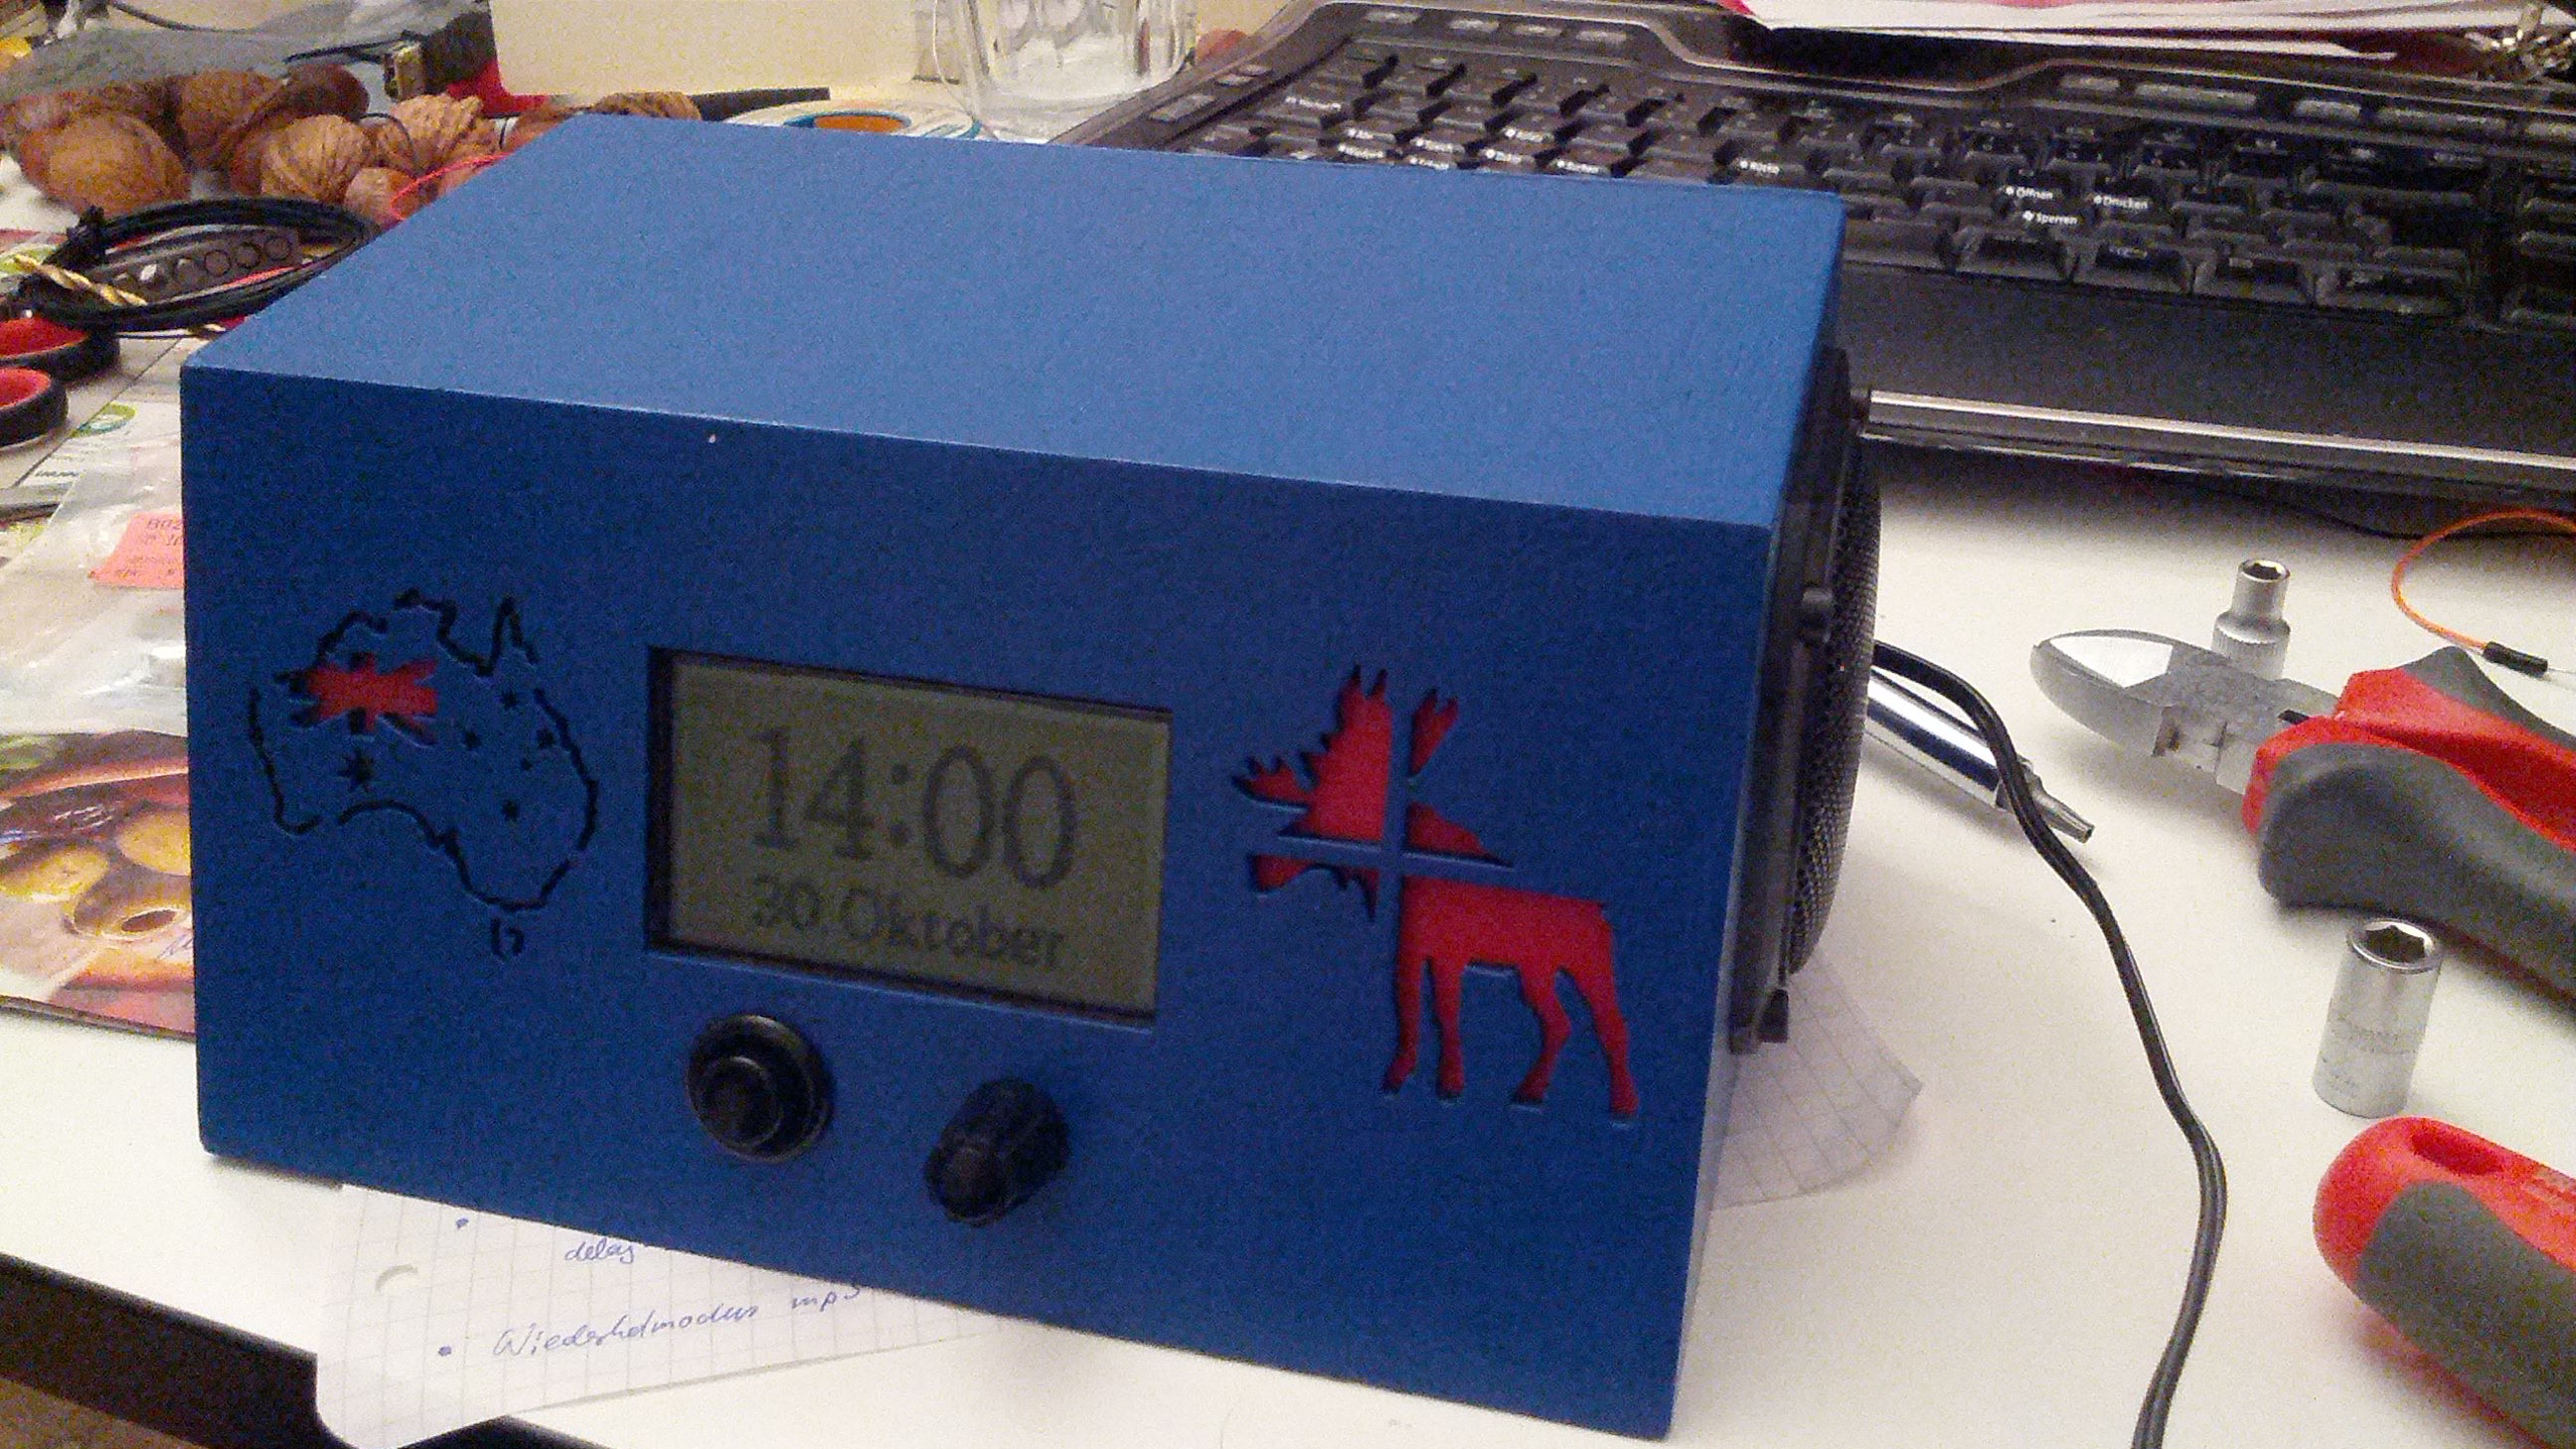
\includegraphics[width=8cm]{./Grafiken/wecker1.jpeg}
		\caption{Wecker bei ausgeschalteter Beleuchtung}
		\label{fig:wecker1}
	\end{center}
\end{figure}
\begin{figure}
	\begin{center}	
		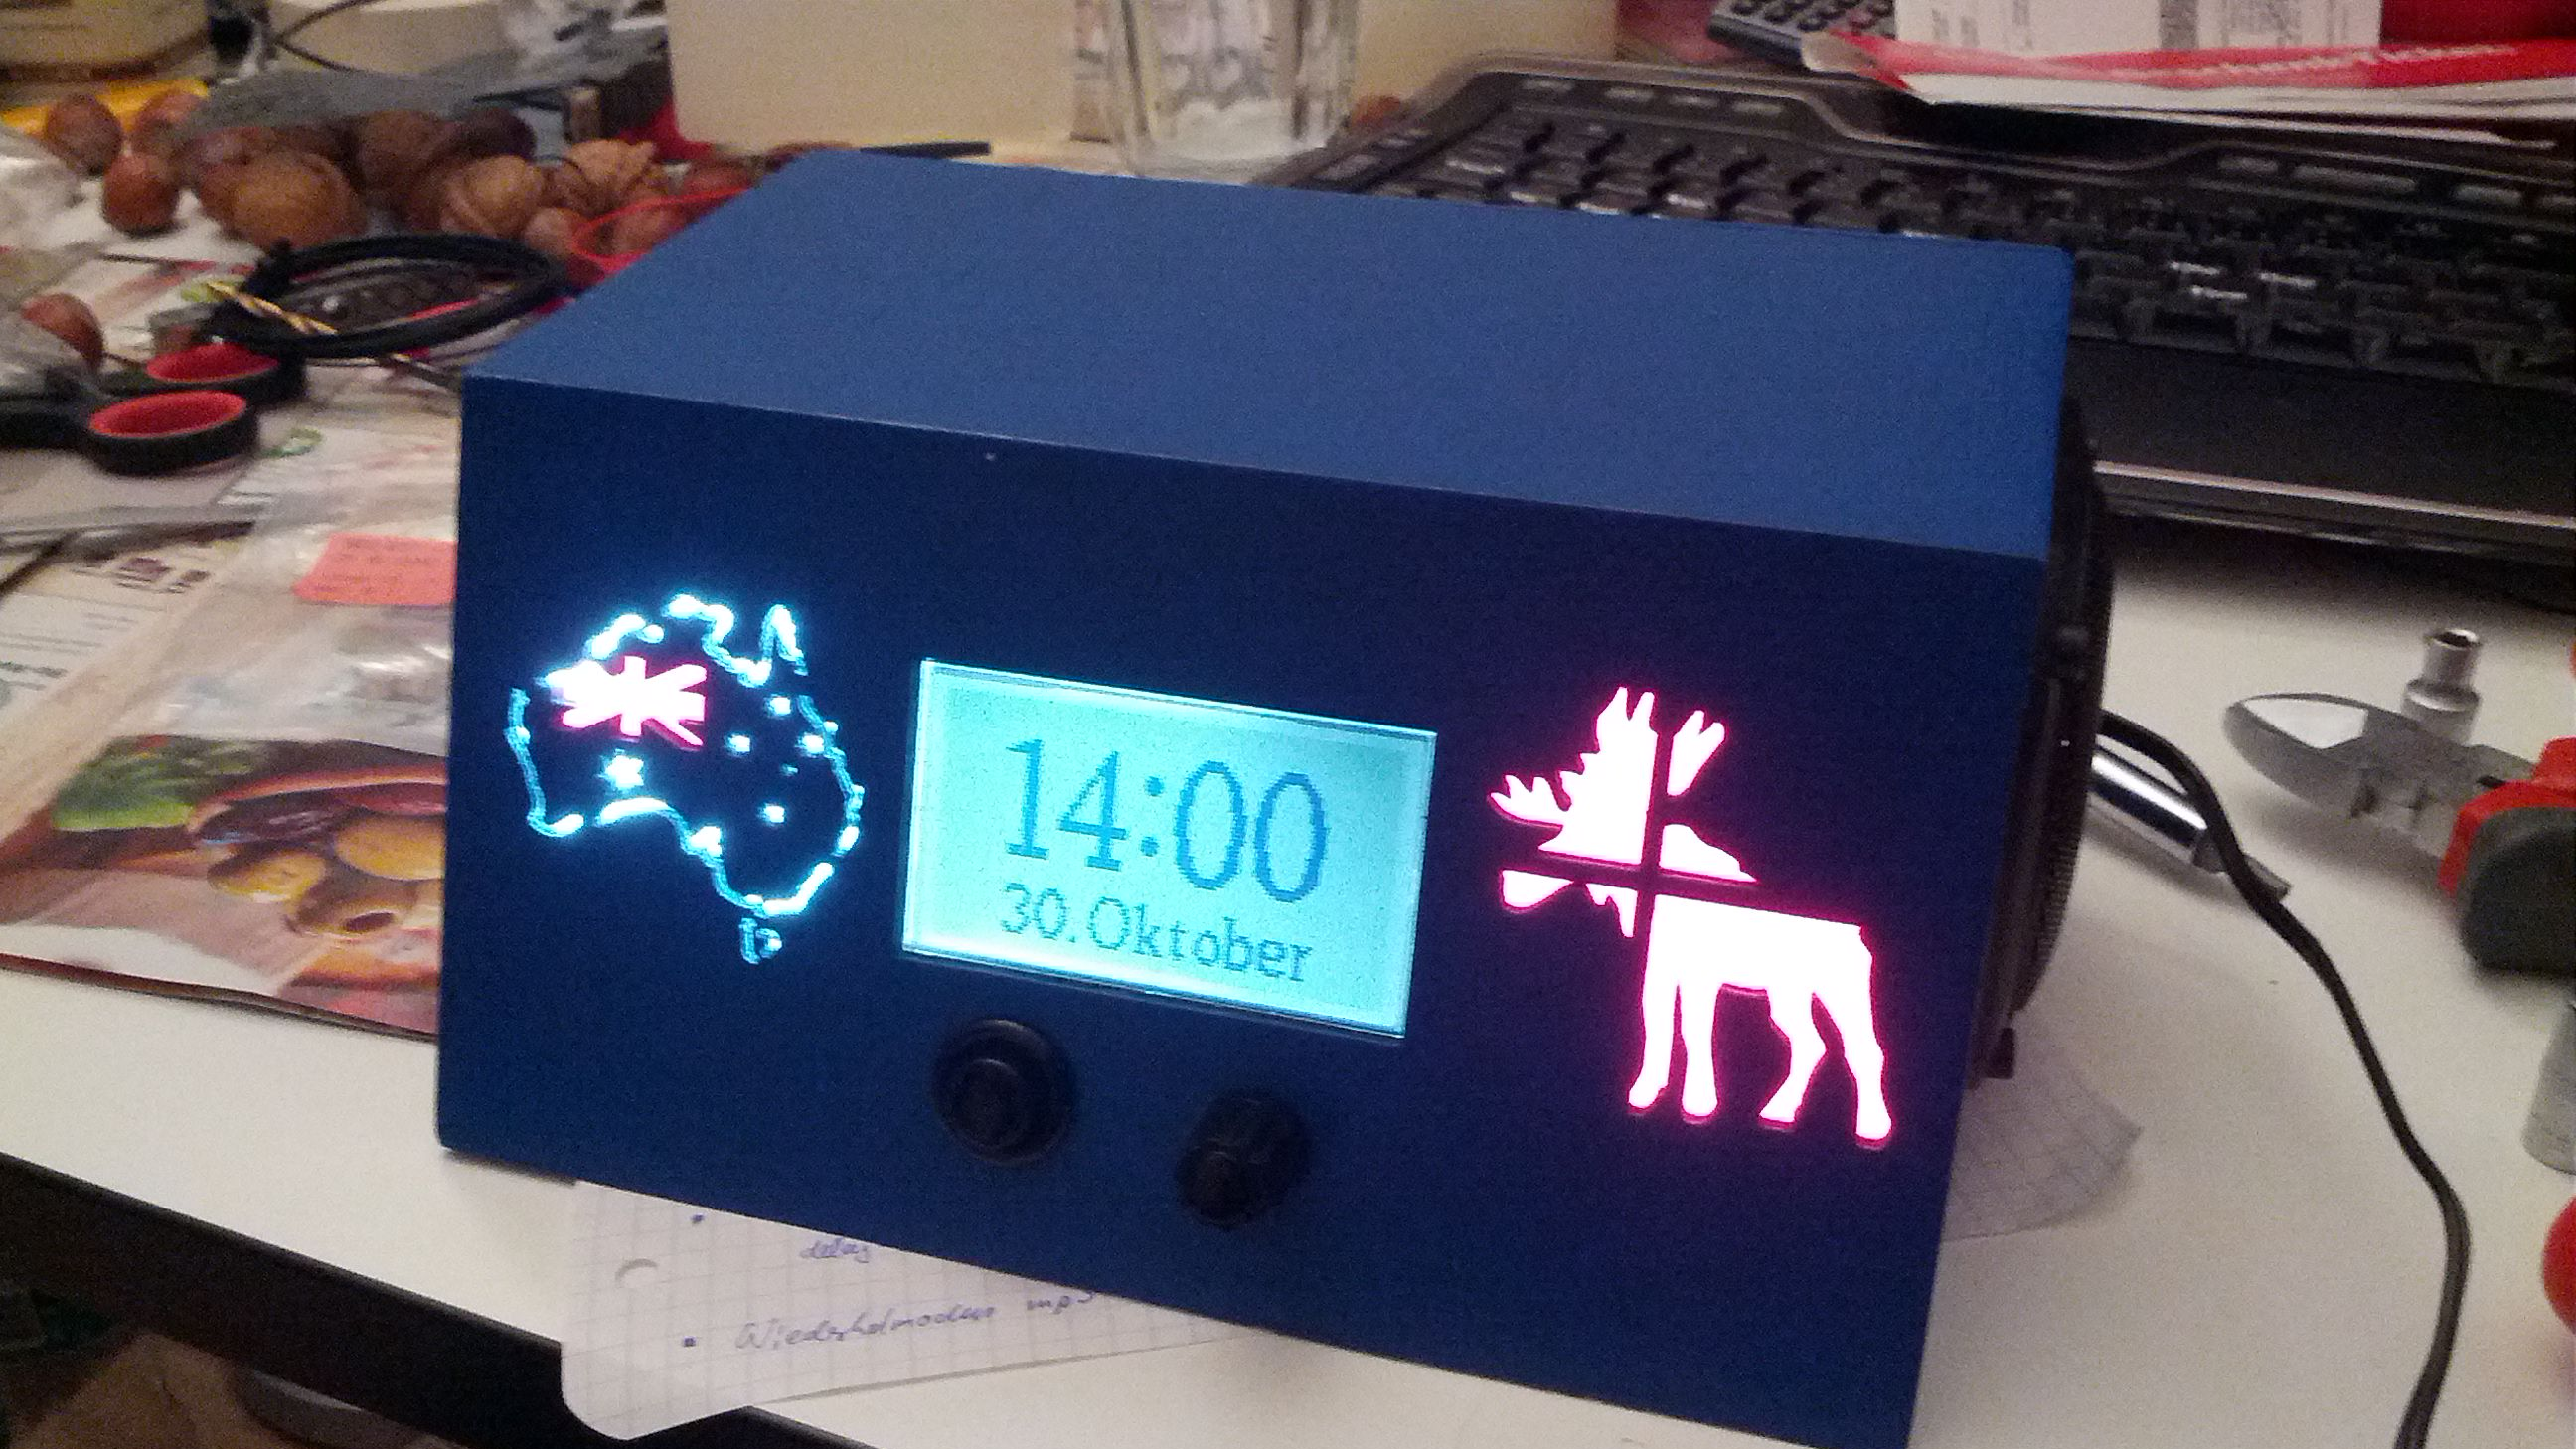
\includegraphics[width=8cm]{./Grafiken/wecker2.jpeg}
		\caption{Wecker bei eingeschalteter Beleuchtung}
		\label{fig:wecker2}
	\end{center}
\end{figure}

\subsection{Alarm}
Um den Alarm ein- oder auszuschalten wird der Taster für mindestens $1,5s$ gedrückt. Ausschalten des Alarms sowie stoppen des Weckrufs geschieht durch Betätigung des Tasters von $1,5s$ oder mehr. Während des Weckrufs ist es außerdem möglich, in den snooze-Modus zu wechseln. Dies geschieht durch kurzes Drücken des Tasters oder Drehen des Drehencoders. Ein erneuter Weckeruf wird nach der im Menü eingestellten Snoozedauer (in Minuten) gestartet. Erneutes snoozen ist nicht möglich und der Weckruf muss über ein $1,5$-sekundiges Drücken des Tasters ausgeschaltet werden.
\subsection{Menü}
Das Menü kann über ein langes Drücken des Drehencoders aufgerufen werden. Navigiert wird über die Drehung desselben. Soll ein Punkt im Menü aufgerufen wird, so muss die Auswahl durch kurzes Drücken auf den Drehencoder getätigt werden. In Untermenüs wie beispielsweise der Uhrzeiteinstellung wird ebenfalls durch eine Drehung navigiert. Soll zum Beispiel die Stunde verändert werden, muss die Markierung über das entsprechende Element navigiert werden. Nach einer Bestätigung durch erneut kurzes Drücken ändert sich das Navigationssymbol und die Stunde der Uhrzeit kann verändert werden. Durch erneutes Drücken des Drehencoders wird dieser Modus verlassen. Das Untermenü kann über den angezeigten Haken verlassen werden.
\subsection{Lautstärke}
Für die Einstellung der Lautstärke des Weckrufs muss der entsprechende Unterpunkt im Menü aufgerufen werden. Daraufhin werden Verstärker und mp3-Player eingeschaltet. Letzterer benötigt etwa zehn Sekunden. Während dieser Zeit erscheint der Schriftzug \emph{\glqq Bitte warten\grqq}. Die Musik geht an und anstatt des Schriftzugs erscheint ein Lautsprecher-Symbol. Die Lautstärke kann nun mittels Drehencoder verstellt werden.
\subsection{Boombox}
Bei Auswahl des Menüpunktes Boombox, wird der Verstärker eingeschaltet. Nun kann über die Cinch-Buchsen und ein entsprechendes Kabel (z.B. $3,5mm$-Klinke $\leftrightarrow$ Cinch) eine externe Audioquelle wie ein Handy oder Laptop angeschlossen werden. Dessen Audiosignal wird dann über die Lautsprecher wiedergegeben.
	

\section{Fazit}
Im Rahmen dieses Projektes sind mehrere lehrreiche Momente aufgetreten. Es beginnt bei dem Einkauf von Bauteilen. Hierbei sollte man direkt das Datenblatt aufrufen und nach einer beispielhaften Beschaltung (Application Circuit) suchen. Diese sollte dann auf das vorliegende Projekt angepasst werden, sodass benötigte Zusatzelemente wie zum Beispiel Kondensatoren ebenfalls eingekauft werden, falls sie nicht vorhanden sind. So können unnötige Zeiten von Stillstand im Projekt vermieden werden.\\
Bei der Erstellung des PCB-Layouts für die Platinen wurde zu Beginn nicht durchgängig die Anordnung der Bauteile auf dem Schaltplan beachtet. Somit kommt es in dem Layout zu viele Kreuzungen der Leiterbahnen. Eine Vorsortierung in Bauteilgruppen erleichtert das Routing und ist deshalb ratsam.\\
Außerdem habe ich meine Kenntnisse im Bereich der Programmierung von Mikrocontrollern ausgebaut. So kann ich jetzt deutlich schneller Timer und Interrupts konfigurieren, weil mir die Struktur der Mikrocontroller verständlicher geworden ist. Hierbei helfen Datenblätter und Application Notes. Das Studieren dieser kann nicht nur im Falle von Mikrocontroller sehr hilfreich sein und so ist es nützlich gelernt zu haben, wie man sich in solchen Dokumenten zurechtfindet.\\
Weiterhin haben viele Gespräche mit anderen Personen gute Ideen zu Tage gefördert und vor allem hilfreiche Verbesserungsvorschläge geliefert. Der Austausch mit diesen Menschen hat mich in einigen Situationen entscheidend nach vorne gebracht.  
Doch das beste Ergebnis ist, dass das Endprodukt der Beschenkten gefällt.


\bibliographystyle{IEEEtran}
\bibliography{IEEEabrv,./References.bib}

\end{document}
